\setcounter{secnumdepth}{-1} 

\newcommand{\num}[1]{\begin{align} #1 \end{align}}
\newcommand{\de}[1]{\stackrel{#1}{=}} 
\newcommand{\impl}[0]{\rightarrow}

\newcommand{\n}{\mathbb{N}}
\newcommand{\s}{\mathbb{S}} 
\newcommand{\bsa}{\underline{\leftrightarrow}}
%\newcommand{\bsa}{\leftrightarroweq}
\newcommand{\mea}{\leftrightsquigarrow}
\newcommand{\el}{\exists}
\newcommand{\ab}{\forall}
\newcommand{\pair}[1][x,y]{ (#1)}
\newcommand*\from{\colon}
\renewcommand{\P}{\mathcal{P}}
\newcommand{\K}{\mathcal{K}}
\newcommand{\PROP}{\mathsf{P}}
\newcommand{\Plift}{\overline \P}
\newcommand{\Klift}{\overline \K}

\newtheorem{conj}{Conjecture} 
\newtheorem{theorem}{Theorem}[conj] \newtheorem{lemma}[theorem]{Lemma}
\newtheorem{claim}[theorem]{Claim} \newtheorem{fact}[theorem]{Fact}
\newtheorem{corollary}[theorem]{Corollary}
 
\newtheorem{notation}[theorem]{Notation}





\subsection{$BML(P):$}
\label{sec:mlp}
\[\phi ::= p \mid \neg p \mid \bot \mid \top \mid \phi \lor \phi \mid \phi \land \phi \mid \Diamond\phi \mid \Box\phi\]

-No problem that the negation is at the propositional letters, as we can make
the ``negation'' $\sim$ trivially by the normal equivalences $\sim\Box\phi = \Diamond~\phi$ and
similar. 


\subsection{Models}
\label{sec:models}
$\pair[S,\sigma], \sigma \from S \to \P(\PROP)\times\P(S)$, $\sigma^{S}(s) := (\sigma_{v}^{S}(s),\sigma_{R}^{S}(s))$

\subsection{Kripke funktor}
\label{sec:kripke-funktor}
$\K(S) := \P(\PROP) \times \P(S)$

\subsection{Bisumulation}
\label{sec:bisumulation}

Let $\pair[A,\sigma^{A}]$ and $\pair[B,\sigma^{B}]$ be two models
Then a non-empty relation $Z \subseteq A \times B$ is a bisimulation if the following hold, for every
$(a, b ) \in Z$.
\begin{enumerate}
\item[(PROP)] $\sigma^{A}_{v}(a)=\sigma^{B}_{v}(b)$
\item[(FORTH)] For all $a' \in \sigma^{A}_{R}(a)$ there is a $b' \in \sigma^{B}_{R}(b)$ with
  $(a',b') \in \Sigma$.
\item[(BACK)] For all $b' \in \sigma^{B}_{R}(b)$ there is a $a' \in \sigma^{A}_{R}(a)$ with
  $(a',b') \in \Sigma$.
\end{enumerate}

\subsection{Bisimulation via relation lifting}
\label{sec:bisim-via-relat}
\begin{definition}[$\overline \P(Z)$]
  \label{def:1}
  Given a relation $Z \subseteq A \times B$ , define the relation $\Plift Z \subseteq \P A \times \P B$
  as follows :
  \begin{align*}
    \Plift Z := \{(X, X' ) \mid \text{for all } a \in X \text{ there is an } b \in X'
    \text{ with } (a, b ) \in Z \\
    \& \text{ for all } b \in X' \text{ there is an } a \in X \text{ with } (a, b
    ) \in Z\}.
  \end{align*}
\end{definition}
\begin{definition}[$\overline \K(Z)$]
  \label{def:1}
   $\Klift Z \subseteq \K A\times\K B$
  \begin{align*}
    \Klift Z := \{((\pi,X), (\pi',X') ) \mid \pi=\pi' \text{ and } (X,X') \in \Plift Z \}.
  \end{align*}
\end{definition}
The relations $\Klift Z$ and $\Plift Z$ are called the liftings of $Z$.

% We say that $Z \subseteq A \times B$ is full on $A' \in \P A$ and $B' \in \P B$ , notation:
% $Z \in A' \bowtie B'$ , if $(A', B') \in \P Z$.

\begin{proposition}
  \label{proof:1}
  Let $\pair[A,\sigma^{A}]$ and $\pair[B,\sigma^{B}]$ be two models, and let $\Sigma \subseteq A \times B$ be some non-empty relation.
  Then
  \[Z \text{ is a bisimulation iff } (\sigma^{A}(a),\sigma^{B}(b))\in \Klift Z \text{ for all }
    (a,b) \in Z.\]
  \end{proposition}

  \subsection{Cover modality}
  \label{sec:cover-modality}
  \begin{definition}
    $S,s \models \nabla\Phi \text{ iff } (\sigma_{R}(s),\Phi) \in \Plift(\models_{S})$\label{def:2}
  \end{definition}
  \[\nabla\Phi \equiv \Box\bigvee\Phi \land \bigwedge \Diamond\Phi  \]
  \[\Diamond \phi \equiv \nabla\{\phi,\top\}\]
  \[\Box \phi \equiv \nabla\emptyset \lor \nabla\{\phi\} \]

  \subsection{BML$_\nabla$}
  \[\phi ::= p \mid \neg p \mid \bot \mid \top \mid \phi \lor \phi \mid \phi \land \phi \mid \nabla\phi\]
  BML$_\nabla$ and BML are equally expressive!

  \subsection{CML}
  \label{sec:cml}
  For finite $\PROP$, and $\pi \subseteq \PROP$:
  \[S,s \models \odot \pi \text{ iff } \sigma_{v}(s) = \pi\]
  \[\odot \pi := \bigwedge_{p \in \pi}p \land \bigwedge_{p \notin \pi} \neg p\]
  \[q \equiv \bigvee_{q \in \pi} \odot \pi\]
  \[\pi \bullet \Phi \equiv \odot\pi \land \nabla\Phi\]

  CML:
  \[\phi ::= \bot \mid \top \mid \phi \lor \phi \mid \phi \land \phi \mid \pi \bullet \Phi\]

  \begin{proposition}
    \label{proof:2}
    $S,s \models \pi \bullet \Phi$ iff $(\sigma(s),(\pi,\Phi)) \in \Klift(\models_{S})$
  \end{proposition}

  \begin{theorem}
    \label{thr:1}
    BML$_\nabla$ and CML are equally expressive. CML to BML$_\nabla$ is trivial by the
    above. For the other way note the two equivalences:
    \[\top \equiv \nabla\emptyset \lor \nabla\{\top\}\]
    \[\top \equiv \bigvee_{\pi \subseteq \PROP} \odot\pi\]

    \begin{align*}
      \odot\pi \equiv& \odot\pi \land \top\\
      \equiv& \odot\pi \land (\nabla\emptyset \lor \nabla\{\top\})\\
      \equiv& (\pi \bullet \emptyset) \lor (\pi \bullet \{\top\})
    \end{align*}

  \end{theorem}

  \subsubsection{CML$^-$}
  \label{sec:cml-1}
  \[\phi ::= \bot \mid \top \mid \phi \lor \phi \mid \pi \bullet \Phi\]

  \begin{theorem}
    \label{thr:2}
    CML and CML$^-$ are expressively equivalent.
  \end{theorem}
  
\section{Part two, modal $\mu$-calculus}
\label{sec:part-two}
$\mu BML(P)$ (or $\mu PML(D,P)$ with many relations $D$.)
\[\phi ::= \bot \mid \top \mid p \mid \neg p \mid \phi \lor \phi \mid \phi \land \phi \mid \Diamond\phi \mid \Box\phi  \mid \mu x.\phi  \mid \nu x.\phi   \]
$p,x \in \PROP$. No $x$ under the scope of a negation. Will write $\eta x.\phi$ for
$\eta$ being $\mu$ or $\nu$. We use $FV(\phi)$ for the free variables (not bound by $\mu$ or
$\nu$), and $BV(\phi)$ for the bounded variables.

\subsubsection{Subformula}
\label{sec:subformula}
$\phi \trianglelefteq \psi$ iff $\phi$ is a subformulae of $\psi$.

\subsubsection{Clean formulae}
\label{sec:clean-formulae}
$x \lor \mu x.((p \lor x) \land \Box\nu x.\Diamond x)$.

\begin{definition}[Clean]
  \label{def:3}
  A formula $\phi$ is clean if no two distinct (occurrences of) fixed point
  operators in $\phi$ bind the same variable, and no variable has both free and
  bound occurrences in $\phi$. If x is a bound variable of the clean formula
  $\phi$, we let $\phi_{x} = \eta_{x} x.\delta_{x}$ denote the unique subformula
  of $\phi$ where x is bound by the fixpoint operator $\eta_{x}$.
\end{definition}

\begin{definition}
  \label{def:4}
   Given a clean formula $\phi$, we define a dependency order on the bounded
   variables of $\phi$, saying that $y$ ranks higher than $x$, notation:  $x\leq_{\phi}y$
   iff $\phi_{x} \trianglelefteq \phi_{y}$.
 \end{definition}

 \subsubsection{Evaluation game}
 \label{sec:evaluation-game}
 Given a formula $\xi$ and a model $\mathbb{S}=(S,\sigma)$ we define the evaluation
 game $\mathcal{E}(\xi,S)$ with the following rules. For a game starting at some
 $s \in S$ we write $\mathcal{E}(\xi,S)@(\xi,s)$.
 \begin{table}[h!]
   \centering
   \begin{tabular}{|l|c|l|}
     \hline Position & Player & Addmissible moves \\\hline
     ($\phi_{1} \lor \phi_{2}$, s)                          &  $\exists$ &  $\{(\phi_{1}, s), (\phi_{2}, s)\}   $\\
     ($\phi_{1} \land \phi_{2}$, s)                          &  $\forall$ &  $\{(\phi_{1}, s), (\phi_{2}, s)\}    $\\
     ($\Diamond \phi$, s)                              &  $\exists$ & $\{(\phi, t) \mid t \in \sigma(s)\} $\\
     ($\Box \phi$, s)                              &  $\forall$ & $\{(\phi, t) \mid t \in \sigma(s)\} $\\\hline
     ($\bot$, s)                                 &  $\exists$ &  $\emptyset $                   \\
     ($\top$ , s)                                 &  $\forall$ &  $\emptyset $                   \\\hline
     $(p, s),$ with p $\in FV (\xi)$ and  $p \in \sigma_{V}(s)$  &  $\forall$ &  $\emptyset $                   \\
     $(p, s),$ with p $\in FV (\xi)$ and $p \notin \sigma_{V}(s)$  &  $\exists$ &  $\emptyset $                   \\
     $(\neg p, s),$ with p $\in FV (\xi)$ and $p \in \sigma_{V}(s)$ &  $\exists$ &  $\emptyset $                   \\
     $(\neg p, s),$ with p $\in FV (\xi)$ and $p \notin \sigma_{V}(s)$ &  $\forall$ &  $\emptyset $                   \\\hline
     $(\eta_{x}x.\delta_{x} ,s)$                          &  $-$ &  ${(\delta_{x}, s)}$           \\
     $(x, s),$ with $x \in BV(\xi)$                &  $-$ &  ${(\delta_{x}, s)}$
     \\
     \hline
   \end{tabular}
   \caption{Evaluation game for modal $\mu$ calculus.}
   \label{not:evalgame}
 \end{table}

\subsubsection{Example formula}
\label{sec:example-formula}
\[\phi= \eta x.p \lor \Box x\]
 \begin{figure}[h!]
   \centering
   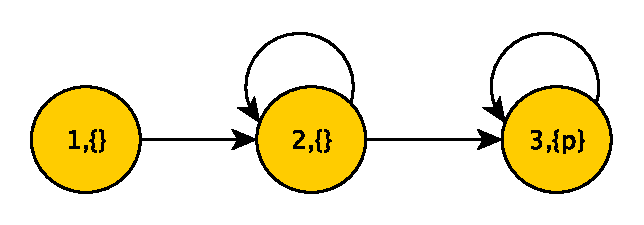
\includegraphics[scale=.8]{smalmoddel}
   \caption{A small model}
 \end{figure}

 \subsubsection{Winning condition in infinite matches}
 \label{sec:winn-cond-infin}
 \begin{definition}
   \label{def:5}
   Given some infinite match $\pi$ on a formula $\xi$ we let
   $Unf^{\infty}(\pi)\subseteq BV(\xi) $ denote the set of variables that are
   unfolded infinitely many times in $\pi$.
 \end{definition}
 Note: For any clean $\xi$ and infinite match $\pi$: the ranking of
 $Unf^{\infty}(\pi)$ according to $\trianglelefteq$ gives a unique highest
 element.


   \begin{table}[h!]
     \centering
     \begin{tabular}{|l|c|c|}
       \hline       & $\exists$ wins $\pi$ & $\forall$ wins $\pi$ \\ \hline
       $\pi$ is finite & $\forall$ got stuck & $\exists$ got stuck\\
       $\pi$ is infinite & max($Unf^{\infty}(\pi)$) is a $\nu$-variable & max($Unf^{\infty}(\pi)$) is a $\mu$-variable  \\\hline    
     \end{tabular}
     \caption{Winning conditions for $\pi$}
     \label{not:winningconditions}
   \end{table}
   \begin{definition}[$Win_{\exists}(\mathcal{E}(\xi,\mathbb{S}))$]
     \label{def:6}
     Let $Win_{\exists}(\mathcal{E}(\xi,\mathbb{S})) \subseteq S$ be all the states in $\mathbb
     S$ such that $\exists$ has a winning strategy.
   \end{definition}
   \begin{definition}
     \label{def:7}
     $(\mathbb{S},s)\models \xi $ iff $(s,\xi) \in Win_{\exists}(\mathcal{E}(\xi,\mathbb{S})).$
   \end{definition}

\section{Exercise 2} 
My formula is the following:
$$\varphi(p,q) = \mu x.((q \land \diamond x)\lor p)$$

I will now prove that $\s,s_0 \vDash \varphi(p,q)$ iff there is a path $s_0Rs_1
\dots Rs_n$ such that $\s,s_n \vDash p$  and $\s,s_i \vDash q$ for all i with $0
\leq i < n$. To make references easier I will name different parts of the
formula, in the same way as was done in exercise 3. 
\begin{align*}
\delta=&((q \land \diamond x)\lor p)\\
\alpha_0=&(q \land \diamond x)\\
\alpha_1=&p
\end{align*}


\begin{theorem}
 $\s,s_0 \vDash \varphi(p,q) \implies$ there is a path $s_0Rs_1
\dots Rs_n$ such that $\s,s_n \vDash p$  and $\s,s_i \vDash q$ for all i with $0\leq i < n$
\end{theorem}
\begin{proof}
  I shall prove the contrapositive. So let us assume that there is no path $s_0Rs_1
\dots Rs_n$ such that $\s,s_n \vDash p$  and $\s,s_i \vDash q$ for all i with
$0\leq i < n$, and lets make sure that $\el$ has no wining strategy.

From our assumption we know that $s_0$ can't satisfy $p$. As $(\delta,s_0)$ is
$\el$'s move, she will then chose $\alpha_0$. Now, if $q$ is false in $s_0$ then
$\ab$ wins, so let us assume otherwise. Then $\ab$ must chose $\diamond x$, and $\el$
can chose a successor. But now notice that as $s_0$ satisfied $q$, none of the
accessible states can satisfy $p$ (because then we would have just the chain that
we assumed that we did not have). $\el$ is then back in a comparable situation
to the one she was in  $(\delta,s_0)$. Again if she chooses $\alpha_1$ she
looses, so she chooses $\alpha_0$. And again, if $q$ is false then $\ab$ wins,
and if $q$ is true then it is again $\el$'s turn to pick a successor. And again,
by the assumption, none of the successors satisfy $p$. 

Two outcomes are
possible. Either we will finally arrive at a state that does not satisfy $q$, and
$\ab$ wins. Or the match will continue forever. But as $x$ is a $\mu$
variable, that also means that $\ab$ wins.

\end{proof}

\begin{theorem}
 There is a path $s_0Rs_1 \dots Rs_n$ such that $\s,s_n \vDash p$  and $\s,s_i
 \vDash q$ for all i with $0\leq i < n$ $\implies \s,s_0 \vDash \varphi(p,q)$
\end{theorem}

\begin{proof}
  I will give a winning strategy for $\el$ in this game given a path as
  mentioned above. Let us call this path $\chi$. Notice that as $\delta$ is a
  disjunction, $(\delta,s_0)$ is $\el$'s move. She will then proceed with the following
  strategy:
  \begin{list}{}{}
  \item If $i<n$: She chooses $\alpha_1$, and then it is $\ab$'s turn. As q by assumption is true in $s_i$,
    if $\ab$ chooses $q$ $\el$ wins. If $\ab$ chooses $\diamond x$, $\el$ can chose a
    successor. She then chooses the successor $s_{i+1}$ governed by $\chi$. Then she is back in
    $\delta$, and can follow this strategy from the new state $s_{i+1}$.
  \item If $i=n$: Then she chooses $\alpha_1$, and as $p$ by assumption holds in
    $s_n$, $\ab$ looses.
\end{list}
Notice that if $s_0=s_n$ she will follow the rule for the $s_n$ case and win immediately.
As we know that there is a finite path such as assumed above, we know that we
will eventually arrive in the case where $i=n$, and $\el$ wins.
\end{proof}

\subsection{Fixpoints}
\label{sec:fixpoints}
First define the truth-seth (realization) of $\phi$ in $\mathbb{S}$ as follows:
$\llbracket \phi \rrbracket^{\mathbb{S}} = \{ s \in S \mid \mathbb{S},s \models \phi \}$.

From now on we will assume that models are of the form $\mathbb{S} = (S,V,R)$
where $V \from \PROP \to \P(S)$. It is clear that we can transform back and to the
coalgebraic version. 

Given $\mathbb{S} = (S,V,R)$ we let $\mathbb{S}[x\mapsto X]=(S,V[x\mapsto X],R)$ where
\[V[x\mapsto X](y) :=
\begin{cases}
  V(y) & y\neq x,\\
  X & y=x.
\end{cases}\]
\[\phi^{\mathbb{S}}_{x} \from \P(S) \to \P(S)\]
\[\phi^{\mathbb{S}}_{x}(X) := \llbracket \phi \rrbracket ^{\mathbb{S}[x \mapsto X]}\]
When is $\phi^{\mathbb{S}}_{x}(X) = X$? Such a $X$ is a fixpoint of $\phi^{\mathbb{S}}_{x}$.

Alternatively, $X$ is a fixpoint if $\mathbb{S}[x\mapsto X] \models x \leftrightarrow \phi$.
\begin{align*}
\phi = p \lor x & \text{ then } \phi_{x}^{\mathbb{S}}(X) = \llbracket p \lor x
\rrbracket^{\mathbb{S}[x \mapsto X]} = V(p) \cup X\\
\phi = \neg x & \text{ then } \phi_{x}^{\mathbb{S}}(X) = \llbracket \neg x
\rrbracket^{\mathbb{S}[x \mapsto X]} = S \setminus X\\
% \phi = p \lor \Diamond x & \text{ then } \phi_{x}^{\mathbb{S}}(X) = \llbracket p \lor \Diamond x
% \rrbracket^{\mathbb{S}[x \mapsto X]} = \sigma_{V}(p)\cup  \{s \mid \sigma_{R}(s)
% \cap X \neq \emptyset\}  \\
\phi = \Diamond \neg x & \text{ then } \phi_{x}^{\mathbb{S}}(X) = \llbracket \Diamond \neg x
\rrbracket^{\mathbb{S}[x \mapsto X]} =  \{s \in S \mid \exists s' \in (S \setminus X) \text{ s.t } sRs' \} 
\end{align*}
\begin{enumerate}
\item The sets V (p) and S are fixpoints of $\phi$, as is in fact any X with $V (p) \subseteq X \subseteq S$.
\item  Since we do not consider structures with empty domain, the formula $\neg x$ has no
fixpoints at all. 
\item In e.g the integers, seeing just $n+1$, the two fixpoints are the even or the odds.
\end{enumerate}


\subsection{Algebraic semantic}
\label{sec:algebraic-semantic}

\begin{align*}
  \llbracket \bot \rrbracket^{\mathbb{S}}   =& \emptyset  \\
  \llbracket \top \rrbracket^{\mathbb{S}}  =&  S \\
  \llbracket p \rrbracket^{\mathbb{S}}   =&  V(p) \\
  \llbracket \neg p \rrbracket^{\mathbb{S}}  =& S\setminus V(p) \\
  \llbracket \phi \lor \psi \rrbracket^{\mathbb{S}} =& \llbracket
  \phi\rrbracket^{\mathbb{S}} \cup \llbracket \psi \rrbracket^{\mathbb{S}} \\
  \llbracket \phi \land \psi \rrbracket^{\mathbb{S}} =& \llbracket
  \phi\rrbracket^{\mathbb{S}} \cap \llbracket \psi \rrbracket^{\mathbb{S}} \\
  \llbracket \Diamond\phi \rrbracket^{\mathbb{S}} =& \{s \in S \mid \exists s' \in \llbracket \phi
  \rrbracket^{\mathbb{S}} \text{ s.t } sRs'\}  \\
  \llbracket \Box\phi \rrbracket^{\mathbb{S}}   =& \{s \in S \mid R[s] \subseteq \llbracket \phi \rrbracket^{\mathbb{S}} \} \\
  \llbracket \mu x.\phi \rrbracket^{\mathbb{S}}   =& \bigcap PRE(\phi^{\mathbb{S}}_{x}) = LFP(\phi^{\mathbb{S}}_{x}) \\
  \llbracket \nu x.\phi \rrbracket^{\mathbb{S}} =& \bigcup POS(\phi^{\mathbb{S}}_{x}) =
  GFP(\phi^{\mathbb{S}}_{x})
\end{align*}
For $F\from \P(X)\to \P(X)$ we have:

\begin{itemize}
\item $PRE(F)$ is all $X'\subseteq X$ such that
$F(X')\subseteq X'$.
\item $POS(F)$ is all $X'\subseteq X$ such that
$F(X') \supseteq X'$.
\end{itemize}



\end{document}

%%% Local Variables: 
%%% mode: latex
%%% TeX-master: "coalgrecap""
%%% End: 